\documentclass[a4paper,10pt, notitlepage]{report}
\usepackage[utf8]{inputenc}
\usepackage{natbib}
\usepackage{amssymb}
\usepackage{amsmath}
\usepackage{enumitem}
\usepackage{xcolor}
\usepackage{cancel}
\usepackage{graphicx}
\usepackage{url}
\usepackage[portuguese]{babel}

%%%%%%%%%%%%%%%%%%%% Notation stuff
\newcommand{\pr}{\operatorname{Pr}} %% probability
\newcommand{\vr}{\operatorname{Var}} %% variance
\newcommand{\rs}{X_1, X_2, \ldots, X_n} %%  random sample
\newcommand{\irs}{X_1, X_2, \ldots} %% infinite random sample
\newcommand{\rsd}{x_1, x_2, \ldots, x_n} %%  random sample, realised
\newcommand{\bX}{\boldsymbol{X}} %%  random sample, contracted form (bold)
\newcommand{\bx}{\boldsymbol{x}} %%  random sample, realised, contracted form (bold)
\newcommand{\bT}{\boldsymbol{T}} %%  Statistic, vector form (bold)
\newcommand{\bt}{\boldsymbol{t}} %%  Statistic, realised, vector form (bold)
\newcommand{\emv}{\hat{\theta}_{\text{EMV}}}
\newcommand{\bfZ}{\mathbf{Z}}
% \newcommand{\defeq}{\vcentcolon =}


% Title Page
\title{Primeira avaliação (A1)}
\author{Disciplina: Inferência Estatística \\ Professor: Luiz Max de Carvalho}
\date{20 de Setembro de 2021}

\begin{document}
\maketitle

% \textbf{Data de Entrega: 19 de Agosto de 2020.}

\begin{center}
\fbox{\fbox{\parbox{1.0\textwidth}{\textsf{
    \begin{itemize}
        \item Por favor, entregue um único arquivo PDF;
        \item O tempo para realização da prova é de 4 (quatro) horas, mais vinte minutos para upload do documento para o e-class;
        \item Responda todas as questões sucintamente;
        \item Marque a resposta final claramente com um quadrado, círculo, ou figura geométrica de sua preferência;
        \item A prova vale 80 pontos; a pontuação restante é contada como bônus.
        \item Apenas tente resolver a questão bônus quando tiver resolvido todo o resto.
    \end{itemize}}
}}}
\end{center}

\section*{Dicas}
\begin{itemize}
 \item Se $X$ tem distribuição exponencial com parâmetro $\lambda > 0$, então, para $x>0$ as funções de densidade de probabilidade e densidade acumulada são, respectivamente,
 \begin{align*}
 f_X(x) &= \lambda \exp\left(-\lambda x\right),\\
 F_X(x) &= 1 - \exp(-\lambda x).
 \end{align*}
 \item Se $X$ tem distribuição Gama com parâmetros $\alpha >0$ e $\beta >0$ e f.d.p.,
 $$
 f_X(x) = \frac{\beta^\alpha}{\Gamma(\alpha)} x^{\alpha - 1} \exp(-\beta x),
 $$
 para $x>0$, então $W = 1/X$ tem distribuição Gama-inversa, com f.d.p.
 $$
 f_W(w) = \frac{\beta^\alpha}{\Gamma(\alpha)} w^{-(\alpha + 1)} \exp(-\beta/w),
 $$
 para $w>0$.
 Ademais, $E[W] = \beta/(\alpha - 1)$ e $\vr(W) = \beta^2/[(\alpha-1)^2(\alpha-2)]$.
\item Se $X_i \sim \operatorname{Gama}(\alpha_i, \beta)$, com $\alpha_i >0$  para todo $i$ e $\beta>0$, então $Y = \sum_{i=1}^n X_i$ tem distribuição Gama com parâmetros $\alpha_y = \sum_{i=1}^n \alpha_i$ e $\beta_y = \beta$.
\item Se $X \sim \operatorname{Gama}(\alpha, \beta)$, $Y = cX$ tem distribuição $\operatorname{Gama}(\alpha, \beta/c)$ para $c>0$.
%  \item Se $X$ tem distribuição Beta com parâmetros $\alpha>0$ e $\beta>0$, temos
%  \[f_X(x \mid \alpha, \beta) = \frac{\Gamma(\alpha + \beta)}{\Gamma(\alpha)\Gamma(\beta)} x^{\alpha-1} (1-x)^{\beta-1}.\]
%  Além disso, se $\alpha, \beta > 1$ e $F_X(m) = 1/2$, então $m \approx \frac{\alpha-\frac{1}{3}}{\alpha + \beta - \frac{2}{3}}$;
%  \item Um processo de Poisson com taxa $\lambda$ por unidade de tempo é um processo estocástico que satisfaz:
%  \begin{itemize}
%   \item O número de chegadas num intervalo de tempo $\Delta_t$ tem distribuição Poisson com média $\lambda\Delta_t$.
%   \item Os números de chegadas em qualquer coleção de intervalos disjuntos são independentes.
%  \end{itemize}
%  \item O máximo de uma amostra aleatória $\rs$, em que cada $X_i$ tem f.d.p./f.m.p $f_X$ e c.d.f $F_X$, tem f.d.p./f.m.p $f_M(y) = nf_X(y) \left[F_X(y)\right]^{n-1}$.
 \end{itemize}
 
\newpage

\section*{1. Circling the square.}

Um círculo $C_r$  de raio $r$ é inscrito em uma folha de papel quadrada com lado $b$.
Suponha que desejamos estimar a área $A$ deste círculo.
Para tanto, vamos amostrar vetores aleatórios de uma distribuição uniforme definida sobre a folha de papel e, para estimar a área da circunferência, contar a proporção de vetores caindo dentro e fora de $C_r$ e multiplicar esta proporção pela área total da folha de papel.

\begin{enumerate}[label=\alph*)]
 \item (2,5 pontos) Mostre que se $X$ e $Y$ são variáveis aleatórias i.i.d. com distribuição $\operatorname{Uniforme}(0,b)$, então $(X,Y)$ possui função de densidade de probabilidade constante sobre $(0, b)\times (0,b)$;
 
 \item (7,5 pontos) Você deixa cair grãos de milho sobre a folha e conta quantos deles cairam dentro do círculo e fora do círculo (porém na folha).
    Vamos supor que este mecanismo gera observações i.i.d. uniforme sobre $(0,b)^2$.
    Represente os grãos que caíram sobre a folha através de $(X_1,Y_1),...,(X_n,Y_n)$ e  defina $Z_i = \mathbb{I}((X_i,Y_i)\in C_r)$, $i=1,...,n$ como uma variável indicadora que recebe valor $1$ se o grão está dentro da circunferência.
    Suponha que depois de medir $\boldsymbol{Z}$ você joga fora $\boldsymbol{X}$ e $\boldsymbol{Y}$, isto é, guarda o milho no pote de novo para fazer pipoca mais tarde.
    Construa um modelo estatístico parametrizado pela área, $A$, da circunferência que reflete este experimento.
    Encontre uma estatística suficiente mínima para o parâmetro deste modelo.
    
    \textit{Dica:} desenhe um diagrama e considere as áreas envolvidas (evite \underline{avaliar} integrais!);
    
 \item (5 pontos) Considere $\delta_1(\boldsymbol{Z}) = b^2\bar{Z}_n$.
 Este é um estimador não enviesado da área do círculo?
 \item (5 pontos) Calcule o erro quadrático médio $R(A, \delta_1)$ de $\delta_1$ e discuta como ele se comporta em relação à quantidade de interesse.
 O que acontece com $R(A, \delta_1)$ quando $A$ cresce?
\end{enumerate}

\textcolor{red}{\textbf{Conceitos trabalhados}: Modelo estatístico, suficiência, viés, EQM.}

\textcolor{purple}{\textbf{Nível de dificuldade}: fácil.}

\textcolor{blue}{
\textbf{Resolução:}\footnote{O título é um trocadilho (``Circle `in' the square'') que faz referência ao famoso problema de construir um quadrado com a mesma área de um círculo usando apenas compasso e régua:~\url{https://en.wikipedia.org/wiki/Squaring_the_circle}.}
Para responder a) basta notar que $X$ e $Y$ i.i.d implica
$$
f_{X,Y}(x, y) = f_X(x)f_Y(y) = \begin{cases}
                                \frac{1}{b^2},\: x, y \in (0, b),\\
     0,\:\text{caso contrário},
                               \end{cases}
$$
que é constante em $(0, b) \times (0, b)$.
Para responder b) temos que encontrar $\eta = \pr(Z_i = 1)$ e então nosso modelo estatístico será $Z_i \sim \operatorname{Bernoulli}(\eta(A))$, isto é, a probabilidade de $Z_i = 1$ depende de $A$ de acordo com uma função conhecida da área $A$, que é a quantidade de interesse.
Vamos mostrar duas maneiras de computar $\eta$ com \textbf{forte} preferência pela maneira mais simples.
Sabemos que para qualquer variável aleatória cuja distribuição tenha pdf $f$, vale
$$
\pr(X \in C) = \int_{C} f(x)\,dx.
$$
Logo, concluímos que
$$
\pr(Z_i = 1) = \int_{C_r} f_{X, Y}(x, y)\,dxdy = \frac{\pi r^2}{b^2}.
$$
isto é, a razão entre área do círculo e do quadrado.
Desta forma, $\eta(A) = A/b^2$.
Agora vamos discutir uma solução bem mais trabalhosa para o problema.
Note que 
$$
\pr(Z_i = 1) = \pr((X_i, Y_i) \in C_r) = \pr(X_i^2 + Y_i^2 \leq r^2).
$$
Sem perda de generalidade, vamos centrar $C_r$ em $(b/2, b/2)$.
Se definirmos  $U = (X_i-b/2)^2$, $V=(Y_i-b/2)^2$ e $T = U + V$, temos que
$$
\pr(Z_i = 1) = F_T(r^2).
$$
Lembrando da fórmula para convolução (soma) de duas v.a.s independentes, temos
$$
F_T(t) = \int_{-\infty}^\infty F_U(t-v)f_V(v)\,dv.
$$
Para computar $F_U$, fazemos
\begin{align*}
 \pr(U \leq u) &= \pr( (X_i-b/2)^2 \leq u),\\
 &= \pr(|X_i-b/2| \leq \sqrt{u}) = 2F_X(\sqrt{u}),\\
 &= 2\frac{\sqrt{u}}{b}
\end{align*}
o que também significa que $f_V(v) = 1/\sqrt{v}$ porque $U$ e $V$ são i.i.d.
Juntando tudo, temos
\begin{align*}
 F_T(t) &= \int_{0}^{\frac{b^2}{4}}  2\frac{\sqrt{t-v}}{b\sqrt{v}} \,dv ,\\
 &= \Re \left(\frac{2}{b^2} \left\{ \dfrac{b\sqrt{4t-b^2}-4t\arctan\left(\frac{\sqrt{4t-b^2}}{b}\right)}{4}+\dfrac{{\pi}t}{2} \right\} \right),\\
 &= \frac{\pi t}{b^2},
\end{align*}
onde $\Re(a + bi)= a$ denota a parte real e $\arctan(x) = y$ se $\tan(y) = x$.
A última linha segue do fato de que $\Re(\sqrt{4r^2-b^2}) = 0$ para $r \in (0, b/2)$, isto é, para os círculos que nos interessam aqui.
Avaliar $F_T(r^2)$ completa a computação necessária.
\textbf{Eu avisei que era melhor evitar computar integrais!}
\\
Vamos mostrar que a soma é suficiente mínima neste exemplo.
Para encontrar uma estatística suficiente, vamos utilizar o teorema da fatorização\footnote{Também chamado de Teorema da Fatorização de Neyman-Fisher, ou NFFT na sigla em inglês.}:
\begin{align*}
f_n\left(\boldsymbol{Z} \mid \eta(A)\right) &= \prod_{i=1}^n \eta(A)^{z_i} \left(1-\eta(A)\right)^{1-z_i},\\
&= \eta(A)^S \left(1-\eta(A)\right)^{n-S},
\end{align*}
com $S = \sum_{i=1}^n z_i$.
Daí, vemos que podemos fatorar a densidade condicional conjunta em $u(\eta(A)) = 1 $ e $v[S, \eta(A)] = \eta(A)^S \left(1-\eta(A)\right)^{n-S}$  e portanto $S$ é suficiente para $\eta(A)$.
Para mostrar que $S$ é suficiente \textbf{mínima}, vamos considerar uma estatística suficiente $T(\boldsymbol{Z})$ de modo que possamos escrever
$$
f_n\left(\boldsymbol{Z} \mid \eta(A)\right) = g[T, \eta(A)]h(\eta(A)).
$$
Agora, tome $A_1 \neq A_2$ e faça
\begin{align*}
% \frac{v[S, \eta(A_1)]u(\eta(A_1))}{v[S, \eta(A_2)]u(\eta(A_2))} &= \frac{g[S, \eta(A_1)]h(\eta(A_1))}{g[S, \eta(A_2)]h(\eta(A_2))},\\
\frac{ \eta(A_1)^S \left(1-\eta(A_1)\right)^{n-S}}{ \eta(A_2)^S \left(1-\eta(A_2)\right)^{n-S}} &= \frac{g[T, \eta(A_1)]h(\eta(A_1))}{g[T, \eta(A_2)]h(\eta(A_2))},\\
\left(\frac{\eta(A_1)\left[1-\eta(A_2)\right]}{\eta(A_2)\left[1-\eta(A_1)\right]}\right)^S\left(\frac{\left(1-\eta(A_1)\right)}{\left(1-\eta(A_2)\right)}\right)^n &= \frac{g[T, \eta(A_1)]h(\eta(A_1))}{g[T, \eta(A_2)]h(\eta(A_2))},
\end{align*}
de onde obtemos
$$
S = f(T) =\frac{\log \left( \frac{g[T, \eta(A_1)]h(\eta(A_1))}{g[T, \eta(A_2)]h(\eta(A_2))}\right) - n\log \left(\frac{\left(1-\eta(A_1)\right)}{\left(1-\eta(A_2)\right)}\right)}{\log \left(\frac{\eta(A_1)\left[1-\eta(A_2)\right]}{\eta(A_2)\left[1-\eta(A_1)\right]}\right) },
$$
e, com isso, mostramos que $S = f(T(\boldsymbol{Z}))$ para toda estatística suficiente $T$, como queríamos.
\\
Outra forma de mostrar que $S$ é suficiente mínima é mostrar que $S$ é uma função bijetiva do EMV $\hat{ p }$ de $p : = \eta ( A )$.
Isso implica em $\hat{ p }$ ser suficiente, o que, pelo Teorema 7.8.3 de DeGroot (Observação 10 dos slides), significa que $\hat{ p }$ é suficiente mínimo e, assim, $S$ também será suficiente mínima, por ser uma função bijetiva de uma estatística suficiente mínima.
Sendo assim, vamos encontrar $\hat{ p }$.
Maximizar $f_{ n } ( \boldsymbol{Z} \mid p )$ é equivalente a maximizar
\begin{equation*}
    G ( p ) : = \log f_{ n } ( \boldsymbol{Z} \mid p ) = S \log p + ( n - S ) \log ( 1 - p ).
\end{equation*}
Derivando, obtemos
\begin{equation*}
    G^\prime ( p ) = \frac{ S }{ p } + \frac{ S - n }{ 1 - p }
\end{equation*}
e
\begin{equation*}
    G^{\prime\prime} ( p ) = - \frac{ S }{ p^2 } + \frac{ S - n }{ ( 1 - p )^2 }.
    \end{equation*}
Como $S \leq n$, temos $G^{\prime\prime}(p) \leq 0$ para todo $p$.
Portanto, $\hat{ p }$ é a solução de $G^\prime(p) = 0$, que podemos, sem muito esforço, identificar como sendo $S/n$.
Dessa forma, temos $S = n \hat{ p }$ e está mostrada a suficiência mínima de $S$.
Agora, vamos trabalhar em c).
Escrever $Z_1, \ldots Z_n \sim \operatorname{Bernoulli}(\eta(A))$ implica
$$
E[\delta_1] = \frac{b^2}{n}E\left[\sum_{i=1}^n Z_i\right] = \frac{b^2}{n} n E[Z_1] = b^2\eta(A) = \pi r^2.
$$
Concluímos portanto que $\delta_1$ é \textbf{não-viesado}.
\\
De c) sabemos que 
\begin{align*}
R(A, \delta_1) &= \vr\left(\delta_1(\boldsymbol{Z})\right),\\
&= \frac{b^4}{n^2}\vr(S) = \frac{b^4n}{n^2}\vr(Z_1),\\
&= \frac{b^4}{n}\left(\frac{A}{b^2}\left(1-\frac{A}{b^2}\right)\right),\\
&= \frac{A(b^2-A)}{n},
\end{align*}
o que responde d).
Note que $\vr(\delta_1)$ é uma função côncava e atinge seu máximo em $A = b^2/2$, que é o ponto médio da amplitude de $A$, $(0, b^2/4)$.
A Figura~\ref{fig:var_delta_1} mostra um esboço de $R(A, \delta_1) = \vr\left(\delta_1\right)$.
\begin{figure}[!ht]
\begin{center}
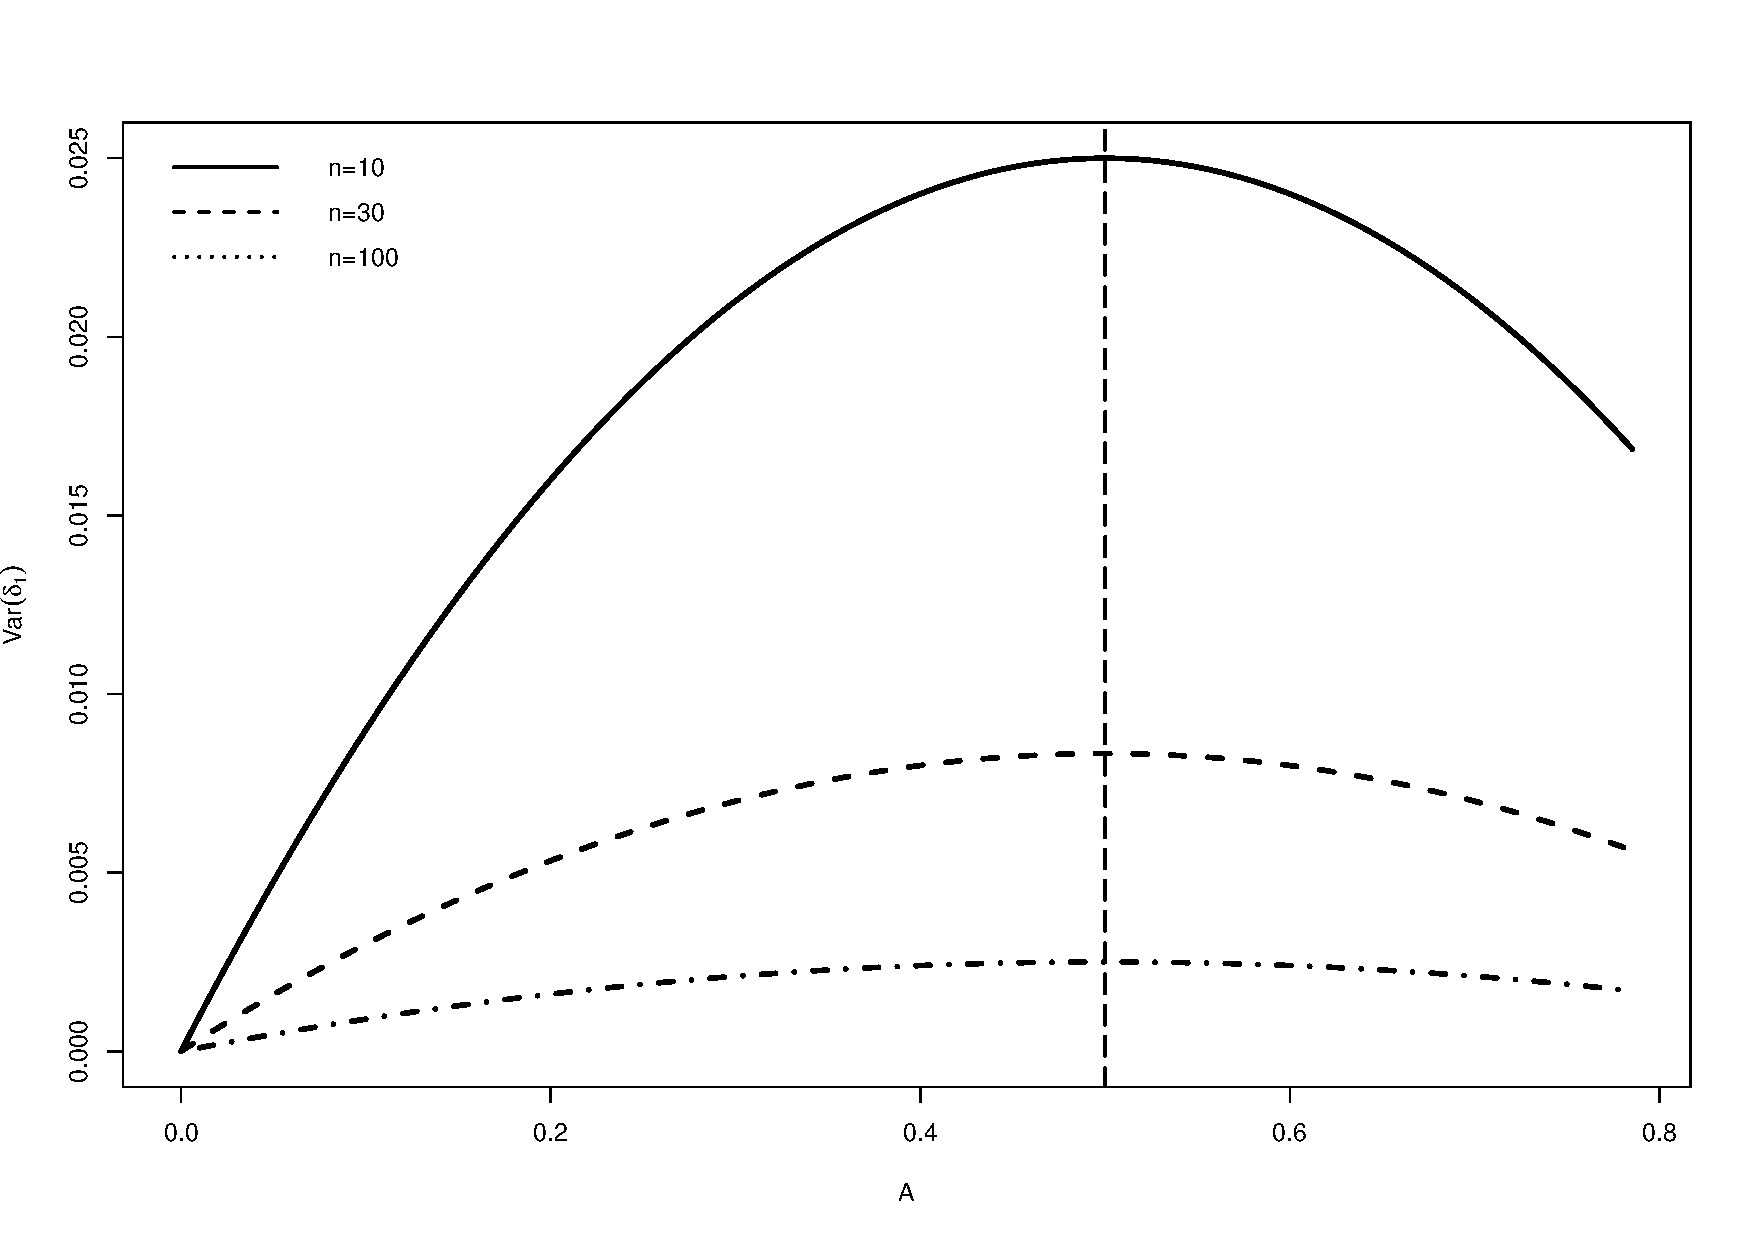
\includegraphics[scale=0.4]{var_delta_1.pdf}    
\end{center}
\caption{\textbf{Erro quadrático médio do estimador $\delta_1$}.
Mostramos a curva para $n=10, 30$ e $100$ com $b=1$.
Note que o máximo é atingido em $(b^2/4 - 0)/2 = b^2/2$.
}
\label{fig:var_delta_1}
\end{figure}
$\blacksquare$
}
\newpage
\section*{2. The shinning.}

Suponha que você é a pessoa responsável pelo controle estatístico de qualidade na fábrica de lâmpadas \textit{LuminaEu}.
Seu chefe, Astolfo, lhe envia uma planilha com os valores $\rs$ dos tempos de falha de $n$ lâmpadas (em dias).
Você lê no manual da empresa que um modelo exponencial i.i.d. com parâmetro $\theta$ é apropriado para análise.

\begin{enumerate}[label=\alph*)]
 \item (5 pontos) Mostre que o estimador de momentos para $\theta$ coincide com o EMV neste caso;
 \item (10 pontos) Discuta se o estimador do item anterior é eficiente para amostras finitas.
 O que acontece assintoticamente?
 \item (5 pontos) Conhecendo Astolfo, no entanto, você sabe que ele não saberá interpretar quaisquer estimativas diretas da taxa $\theta$, então decide considerar a probabilidade de excedência\footnote{Em inglês, \textit{exceedance probability}.} $\alpha := \pr(X_1 > c)$ para um certo $c > 0$.
 Encontre um estimador de máxima verossimilhança para $\alpha$;
\end{enumerate}
\textcolor{red}{\textbf{Conceitos trabalhados}: Método dos momentos, EMV, reparametrização, invariância, eficiência.}
\\
\textcolor{purple}{\textbf{Nível de dificuldade}: fácil.}
\\
\textcolor{blue}{
\textbf{Resolução:}
Sabendo que $E[X_1] = 1/\theta$, o estimador de momentos pode ser obtido escrevendo $\bar{x}_n = 1/\theta$ o que nos leva a $\hat{\theta}_{MM} = n/S$, com $S = \sum_{i=1}^n X_i$.
Para o encontrar o EMV, escrevemos
\begin{align*}
 f_n(\boldsymbol{X} \mid \theta)= \theta^n \exp\left(-S\theta\right).
\end{align*}
Tomando o log e diferenciando, temos
\begin{align}
\label{eq:q2:l1}
 \lambda_n^\prime(\boldsymbol{X} \mid \theta) &= \frac{n}{\theta} - S ,\\
 \label{eq:q2:l2}
 \lambda_n^{\prime\prime}(\boldsymbol{X} \mid \theta) &= -\frac{n}{\theta^2},
\end{align}
que nos informam que o problema de otimização é côncavo, o que garante que nosso velho conhecido $\hat{\theta}_{EMV} = n/S = 1/\bar{x}_n$ é o único ponto de máximo e o nosso EMV para $\theta$.
Isso mostra que os estimadores coincidem.
\\
Para entender se $\delta(X)= n/S$ é eficiente, convêm entender primeiro se é viesado. 
Das dicas podemos deduzir que $\delta$ tem distribuição Gamma inversa com parâmetros $\alpha_\delta = n$ e $\beta_\delta = n\theta$, o que nos leva à conclusão de que $E_\theta[\delta] = n/(n-1) \theta$ e portanto $\operatorname{vies}(\delta) = -\theta/(n-1)$.
Das dicas sabemos também que
$$
\vr_\theta(\delta) = \frac{n^2\theta^2}{(n-1)^2(n-2)}.
$$
% portanto
% \begin{align*}
% R(\delta, \theta) &= \frac{n^2\theta^2}{(n-1)^2(n-2)} + \frac{\theta^2}{(n-1)^2},\\
% &= \theta^2\frac{n^2 + n -2}{(n-1)^2(n-2)}.
% \end{align*}
Agora vamos verificar se $\delta$ atinge a cota inferior de Crámer-Rao:
$$
\vr_\theta(\delta) \geq \frac{[m^\prime(\theta)]^2}{nI(\theta)},
$$
onde $m(\theta) := E_\theta[\delta]$ e $I(\theta)$ é a informação de Fisher.
Dos cálculos acima, sabemos que $[m^\prime(\theta)]^2 = n^2/(n-1)^2$.
Para computar $I(\theta)$ vamos nos aproveitar da identidade $I(\theta) = \vr_\theta(\lambda^\prime(x \mid \theta))$:
$$
I(\theta) = \vr_\theta\left(\frac{1}{\theta}  -x\right) = \vr_\theta\left(\frac{1}{\theta}\right) + \vr_\theta\left(-x\right) = 0 + \frac{1}{\theta^2}.
$$
Juntando tudo, temos
$$
\vr_\theta(\delta) \geq \frac{n\theta^2}{(n-1)^2} = V_{\textrm{op}},
$$
o que mostra que $\delta$ está longe de ser eficiente para amostras finitas.
Com efeito, $\vr_\theta(\delta)/V_{\textrm{op}} = n/(n-2)$, o que indica que o EMV e o EMM são assintoticamente eficientes.
\\
Das dicas, sabemos que $\alpha = 1 - F_X(c) = \exp(-\theta c)$, o que nos leva a
\begin{equation}
\label{eq:q2:transf}
\theta = -\log(\alpha)/c. 
\end{equation}
Para responder c) e encontrar o EMV de $\alpha$, temos dois caminhos: (i) lembrar da invariância do EMV, substituir o estimador do item anterior em (\ref{eq:q2:transf}) ou; (ii) reescrever a verossimilhança de acordo com o novo parâmetro (procedimento chamado de~\textit{reparametrização}) e maximizar esta nova função.
Como você deve estar advinhando, aqui vamos fazer as duas coisas.
Fazendo a substituição, temos $\hat{\alpha} = \exp(-\hat{\theta}c) = \exp(-nc/S)$ e, para o caminho (ii):
\begin{align*}
 f_n(\boldsymbol{X} \mid \alpha) &= [-\log(\alpha)/c]^n \exp\left(S\log(\alpha)/c\right),\\
 &\propto [-\log(\alpha)]^n \exp\left(S\log(\alpha)/c\right).
\end{align*}
Fazendo o procedimento usual, temos
\begin{align}
\label{eq:q2:rl1}
 \lambda_n^\prime(\boldsymbol{X} \mid \alpha) &= \frac{n}{\alpha \log(\alpha)} + \frac{S}{c\alpha},\\
 \label{eq:q2:rl2}
 \lambda_n^{\prime\prime}(\boldsymbol{X} \mid \alpha) &= -\frac{n}{\alpha^2\log(\alpha)}-\frac{n}{\alpha^2\log^2(\alpha)}-\frac{S}{c\alpha^2}.
\end{align}
Para começar, vemos que atacar o problema diretamente foi uma má ideia: as equações são mais difíceis de resolver e de verificar.
Não obstante, podemos resolver (\ref{eq:q2:rl1}) e encontrar...
$\hat{\alpha} =  \exp(-nc/S)$, para surpresa de $0$ pessoas!
Isso conclui c).
$\blacksquare$
}

\section*{3. Cool and normal!}

Suponha que você é a pessoa responsável por analisar a concentração de ácido em pedaços de queijo vindos da famosa fábrica de frios francesa \textit{J'skeci}.
Assumindo uma distribuição normal para as concentrações em $n$ medições independentes de $n$ pedaços distintos, você precisa descobrir a média $\mu$ e a variância $v$ desta distribuição.

\begin{enumerate}[label=\alph*)]
 \item (5 pontos) Considere a priori imprópria
 \begin{equation}
 \label{eq:improp_prior}
 \xi(\mu, v) \propto 1/v
 \end{equation}
 Mostre que a posteriori $\xi(\mu, v \mid \boldsymbol{x})$ é própria;
 
 \textit{Dica:} Procure com atenção o núcleo de distribuições conhecidas.
 \item (7,5 pontos) Exiba o estimador de Bayes sob perda quadrática para $v$ e o estimador de Bayes sob perda absoluta para $\mu$ e discuta se esses estimadores são viesados;
 \item (5 pontos) Encontre uma priori  conjugada para $(\mu, v)$;
 \item (2,5 pontos) Mostre que a priori em (\ref{eq:improp_prior}) pode ser vista como um limite particular (dos hiperparâmetros) da priori conjugada do item anterior.
\end{enumerate}
\textcolor{red}{\textbf{Conceitos trabalhados}: Bayes, propriedade, conjugação}
\\
\textcolor{purple}{\textbf{Nível de dificuldade}: médio.}

\textcolor{blue}{
\textbf{Resolução:}
Para começar, vamos escrever a verossimilhança:
\begin{align*}
 f_n(\boldsymbol{x} \mid \mu, v) = \left[\frac{1}{\sqrt{2\pi v}}\right]^n \exp\left(-\frac{1}{2v}\sum_{i=1}^n (x_i -\mu)^2\right).
\end{align*}
Descartando termos que não dependem dos parâmetros de interesse e utilizando a igualdade $\sum_{i=1}^n (x_i -\mu)^2 = \sum_{i=1}^n (x_i -\bar{x}_n)^2 + n(\mu-\bar{x}_n)^2 = s_n^2 + n(\mu-\bar{x}_n)^2$, temos
\begin{align*}
 f_n(\boldsymbol{x} \mid \mu, v) &\propto v^{-n/2} \exp\left(-\frac{1}{2v} \left\{ s_n^2 + n(\mu-\bar{x}_n)^2 \right\}\right),\\
 &\propto \exp\left(-\frac{n(\mu-\bar{x}_n)^2}{2v}\right)v^{-n/2} \exp\left(-\frac{s_n^2}{2v}\right).
\end{align*}
Daí, temos a posteriori
\begin{align}
\nonumber
 \xi(\mu, v \mid \boldsymbol{x}) &\propto f_n(\boldsymbol{x} \mid \mu, v)\xi(\mu, v),\\
 \label{eq:nig_post}
 &\propto \underbrace{\exp\left(-\frac{n(\mu-\bar{x}_n)^2}{2v}\right)}_{\operatorname{Normal}(\bar{x}_n, \frac{v}{n})}\underbrace{v^{-n/2-1} \exp\left(-\frac{s_n^2}{2v}\right)}_{\operatorname{Gama-Inversa}(\frac{n}{2}, \frac{s_n^2}{2})},\\
 \nonumber
 &= p_1(\mu \mid \boldsymbol{x}, v)p_2(v \mid \boldsymbol{x}).
\end{align}
Vemos então que a posteriori se fatora em uma posteriori para $\mu$ condicional a $v$ e aos dados, e uma posteriori marginal (em relação a $\mu$) para $v$.
Com isso, podemos responder b): Para $v$ queremos a média~\textit{a posteriori}, que é o estimador de Bayes sob perda quadrática.
Usando as dicas, sabemos que $E_{p_2}[v] = (s_n^2/2)/((n-2)/2) = s_n^2/(n-2)$.
Já o estimador solicitado para $\mu$ é a mediana~\textit{a posteriori} de acordo com $p_1$, o que é simplesmente $\bar{x}_n$.
Note que este estimador independe do valor de $v$.
Agora podemos dizer que o estimador para $\mu$ é não-viesado, já que $E[\bar{X}_n] = \mu$, e que o estimador para $v$ é viesado, já que o estimador de $v$ não-viesado da forma $\delta_c(\bX) = c \sum_{i=1}^n (X_i -\bar{X}_n)^2$ tem $c = 1/(n-1)$, como visto em aula.
\\
Para responder c) vamos notar que precisamos encontrar $\tilde{\xi}: (-\infty, \infty)\times (0, \infty) \to (0, \infty) \in \mathcal{F}$ de modo que
$$
\exp\left(-\frac{n(\mu-\bar{x}_n)^2}{2v}\right)v^{-n/2} \exp\left(-\frac{s_n^2}{2v}\right)\tilde{\xi}(\mu, v) \in \mathcal{F}.
$$
As derivações acima sugerem uma estrutura condicional para $\tilde{\xi}$ da mesma forma daquela em (\ref{eq:nig_post}): se fizermos $\tilde{\xi}(\mu, v) = \pi_1(\mu \mid v) \pi_2(v)$, podemos escrever:
$$
\tilde{\xi}(\mu, v \mid \boldsymbol{x}) \propto \exp\left(-\frac{n(\mu-\bar{x}_n)^2}{2v}\right)\pi_1(\mu \mid v) \cdot v^{-n/2}\exp\left(-\frac{s_n^2}{2v}\right)\pi_2(v) \in \mathcal{F},
$$
o que nos sugere o sistema de equações funcionais
\begin{align*}
 \exp\left(-\frac{n(\mu-\bar{x}_n)^2}{2v}\right)\pi_1(\mu \mid v)  &= \operatorname{Normal}(m, \tau),\\
 v^{-n/2}\exp\left(-\frac{s_n^2}{2v}\right)\pi_2(v) &= \operatorname{Gama-inversa}(\alpha^\prime, \beta^\prime).
\end{align*}
Para resolver a primeira equação, lembramos que para $v$ fixa, podemos escrever $\pi_1(\mu, v; m, \lambda) = \operatorname{Normal}(m, v/\lambda)$ e, completando o quadrado (duas vezes) vemos que a posteriori resultante continua na família normal (condicional a $v$).
Também podemos ver que $\pi_2(v; \alpha_0, \beta_0) = \operatorname{Gama-inversa}(\alpha_0, \beta_0)$ leva a uma posteriori marginal para $v$ que permanece na família Gama-inversa, o que conclui o nosso argumento.
\\
No que toca à questão d), vamos escrever a densidade conjunta~\textit{a priori}:
$$
\tilde{\xi}(\mu, v) = \frac{\beta_0^{\alpha_0}}{\Gamma(\alpha_0)} v^{-\alpha_0-1}\exp\left(-\beta_0 v\right)\frac{1}{\sqrt{2\pi v}}\exp\left(-\frac{\lambda (\mu-m)^2}{2v}\right).
$$
Para obter $\tilde{\xi}(\mu, v) \propto v^{-1}$, podemos tomar $\beta_0 \to \infty$, $\alpha_0 \to 0$ pelo lado da Gama-inversa e $\lambda \to \infty$ pelo lado da normal.
Desta forma, vemos que, pelo menos neste caso, uma priori imprópria pode ser vista como um limite particular de prioris próprias.
$\blacksquare$
}

\section*{4. Get your ducks in a row.}

Pato Donald, Huguinho, Zezinho e Luisinho estão estudando Inferência Estatística para trabalhar no \textit{hedge fund} do Tio Patinhas.
O problema em questão é a estimação do parâmetro $\theta$ de uma distribuição uniforme em $(\theta/2, 3\theta/2)$ a partir de uma amostra aleatória $\rs$.
Cada um propôs um estimador diferente para $\theta$ e seu trabalho é ajudar o Tio Patinhas a ordenar esses estimadores em ordem de qualidade.

Sejam $M := \max\left(\rs \right)$ e $m := \min\left(\rs\right)$.

Os estimadores escolhidos foram
\begin{enumerate}
% \delta_{\text{}}(\bX)
 \item $\delta_{\text{D}}(\bX) = X_1$, para o Pato Donald;
 \item $\delta_{\text{H}}(\bX) = m$, para Huguinho;
 \item $\delta_{\text{Z}}(\bX) = M$, para Zezinho;
 \item $\delta_{\text{L}}(\bX) = (M+m)/2$, para Luisinho;
\end{enumerate}

Para lhe ajudar na tarefa de julgar estes estimadores, Tio Patinhas enviou o seguinte conjunto de fatos úteis: para $\rs \sim \operatorname{Uniforme}(a, b)$, temos
\begin{align*}
&E[X_1] = \frac{a + b}{2},\\
& \vr(X_1) = \frac{(b-a)^2}{12},\\
&E[m] = a + \frac{1}{n+1}(b-a),\\
&E[M] = b - \frac{1}{n+1}(b-a),\\
&\vr(m) = \vr(M) = \frac{n}{(n+1)^2(n+2)}(b-a)^2,\\
&\operatorname{Cov}\left(m, M\right) = \frac{(b-a)^2}{(n+1)^2(n+2)},\\
&\operatorname{Corr}\left(m, M\right) = \frac{1}{n}.
\end{align*}

Os patos ainda não sabem Inferência Estatística muito bem, portanto tenha paciência com eles.

\begin{enumerate}[label=\alph*)]
 \item (2,5 pontos) Os estimadores de Huguinho e Zezinho são viesados.
 Mostre aos patinhos como construir versões não-viesadas, $\delta_{\text{UH}}(\bX)$ e $\delta_{\text{UZ}}(\bX)$ ;
 \item (2,5  pontos) Discuta se algum dos estimadores do item anterior é inadmissível;
 \item (2,5  pontos) Mostre que $\boldsymbol{T} = (m, M)$ é suficiente conjunta para $\theta$;  
 \item (7,5 pontos) Mostre que $\delta_{\text{L}}(\bX) = E\left[\delta_{\text{D}}(\bX) \mid \boldsymbol{T}\right]$, isto é, que o estimador de Luisinho é o melhoramento de Rao-Blackwell do estimador do Pato Donald;
 \item (5 pontos) Ordene os estimadores $\delta_{\text{D}}(\bX)$, $\delta_{\text{UH}}(\bX)$, $\delta_{\text{UZ}}(\bX)$ e $\delta_{\text{L}}(\bX)$ em termos de erro quadrático médio.
 Quem propôs o melhor estimador?\footnote{No caso de Huguinho e Zezinho, com a sua ajuda.} 
\end{enumerate}
\textcolor{red}{\textbf{Conceitos trabalhados}: Rao-Blackwell, viés, EQM, admissibilidade.}
\\
\textcolor{purple}{\textbf{Nível de dificuldade}: médio.}
\\
\textcolor{blue}{
\textbf{Resolução:} Para começar, vamos nos dar conta de que 
\begin{align*}
 E_\theta\left[\delta_{\text{H}}(\bX)\right] &= \frac{1}{2}\theta + \frac{1}{n+1}\theta = \frac{n+3}{2(n+1)} \theta = k_{\text{H}}\theta,\\
 E_\theta\left[\delta_{\text{Z}}(\bX) \right] &= \frac{3}{2}\theta - \frac{1}{n+1}\theta = \frac{3n + 1}{2(n+1)}\theta = k_{\text{Z}}\theta,
\end{align*}
o que imediatamente sugere
\begin{align*}
 \delta_{\text{UH}}(\bX) &= \frac{1}{k_{\text{H}}}\delta_{\text{H}}(\bX),\\
\delta_{\text{UZ}}(\bX) &= \frac{1}{k_{\text{Z}}}\delta_{\text{Z}}(\bX),
\end{align*}
como soluções de a).
Para reponder b), vamos lembrar que os estimadores são não-viesados e desta forma os EQMs são dados apenas pelas variâncias dos estimadores.
Portanto:
\begin{align*}
R\left(\theta, \delta_{\text{UH}}\right) &= \vr\left(\delta_{\text{UH}}(\bX)\right) = \frac{1}{k_{\text{H}}^2}\vr\left( \delta_{\text{H}}(\bX)\right) = \frac{4(n+1)^2}{(n+3)^2}\vr\left( \delta_{\text{H}}(\bX)\right),\\
R\left(\theta, \delta_{\text{UZ}}\right) &= \vr\left(\delta_{\text{UZ}}(\bX)\right) = \frac{1}{k_{\text{Z}}^2}\vr\left( \delta_{\text{Z}}(\bX)\right) = \frac{4(n+1)^2}{(3n+1)^2}\vr\left( \delta_{\text{H}}(\bX)\right),
\end{align*}
onde a última igualdade da segunda linha vem do fato de que $m$ e $M$ tem a mesma variância. 
Com isso vemos que o estimador de Zezinho domina uniformemente o estimador de Huguinho, que é inadmissível, portanto.
Uma observação interessante, então, é de que, no que toca à tarefa de estimar $\theta$, o máximo da amostra é estritamente mais informativo sobre o parâmetro que o mínimo.
\\
Parte da questão c) foi trabalhada em aula.
Em particular, podemos escrever a verossimilhança como
$$
f_n(\bX \mid \theta) =  \begin{cases}
     \frac{\mathbb{I}\left( m/2 < \theta\right)\mathbb{I}\left(2M/3 < \theta\right)}{\theta^n}, 0 \leq x \leq \theta,\\
     0,\:\text{caso contrário},
\end{cases}
$$
o que mostra que $\boldsymbol{T} = (m, M)$ é suficiente\footnote{Além disso, $\boldsymbol{T}^\prime = (m/2, 2M/3)$ também é suficiente para $\theta$.}, pelo Teorema da Fatorização.
\\
A solução de d) passa por lembrar bem o que é o mecanismo de Rao-Blackwell para melhoramento de estimadores: dado um estimador $\delta$ de $g(\theta)$, e uma estatística suficiente $T$ para $g(\theta)$, podemos sempre construir 
$$
\delta_0 := E_\theta[\delta \mid T],
$$
que domina $\delta$ em termos de EQM.
Com as informações das dicas da questão e do item c), fica claro que estamos procurando $E_\theta[\delta_{\text{D}}(\bX) \mid m, M]$.
Notando que 
$$
f_{1}(x_1 \mid m, M) =  \begin{cases}
     \frac{1}{M-m}, m \leq x_1 \leq M,\\
     0,\:\text{caso contrário},
\end{cases}
$$
isto é que $X_1 \mid m, M \sim \operatorname{Uniforme}(m, M)$, obtemos
\begin{align*}
E_\theta[X_1 \mid m, M] &= E_\theta[\delta_{\text{D}}(\bX) \mid \delta_{\text{H}}(\bX), \delta_{\text{Z}}(\bX)],\\
&= \frac{\delta_{\text{Z}}(\bX)  + \delta_{\text{H}}(\bX)}{2},\\
&= \delta_{\text{L}}(\bX),
\end{align*}
como queríamos demonstrar.
Para finalizar a questão e responder e), precisamos computar o EQM dos estimadores do Pato Donald e de Luisinho.
Para o primeiro, temos:
\begin{align*}
R(\theta, \delta_{\text{D}}(\bX)) &= \vr(X_1) + \left[E[X_1] - \theta\right]^2,\\
&= \frac{\theta^2}{12} + 0 = \frac{1}{12}\theta^2.
\end{align*}
Já para o estimador de Luisinho, temos 
\begin{align*}
E[\delta_{\text{L}}(\bX)] &= \frac{E[m] + E[M]}{2} = \frac{(4n+4)\theta}{4(n+1)} = \theta,\\
\vr\left( \delta_{\text{L}}(\bX) \right) &= \frac{\vr(m) + \vr(M) + 2\operatorname{Cov}(m,M)}{4},\\
&= \frac{\vr(M) + \operatorname{Cov}(m,M)}{2},\\
&= \frac{\theta^2}{2(n+1)(n+2)}.
\end{align*}
Com isso, podemos computar
\begin{align*}
 R(\theta, \delta_{\text{L}}(\bX)) &= \frac{\theta^2}{2(n+1)(n+2)}.
\end{align*}
Agora estamos preparados para construir a nossa ordenação:
\begin{align*}
 R(\theta, \delta_{\text{D}}(\bX)) &= \frac{1}{12}\theta^2,\\
 R(\theta, \delta_{\text{UH}}(\bX)) &= \frac{4n}{(n+3)^2(n+2)}\theta^2,\\
 R(\theta, \delta_{\text{UZ}}(\bX)) &= \frac{4n}{(3n+1)^2(n+2)}\theta^2,\\
 R(\theta, \delta_{\text{L}}(\bX)) &= \frac{1}{2(n+1)(n+2)}\theta^2.
\end{align*}
De modo que \textbf{Zezinho} é o vencedor, com o estimador com menor EQM.
Isso se deve em parte ao fato de que Zezinho utilizou uma estatística suficiente.
Luisinho até foi esperto e usou Rao-Blackwell, mas como o estimador original (do Pato Donald) não era uma estatística suficiente, acabou conseguindo um estimador ruim.
A Figura~\ref{fig:duck_ests} mostra a distribuição dos estimadores considerados aqui.
\begin{figure}[!ht]
\begin{center}
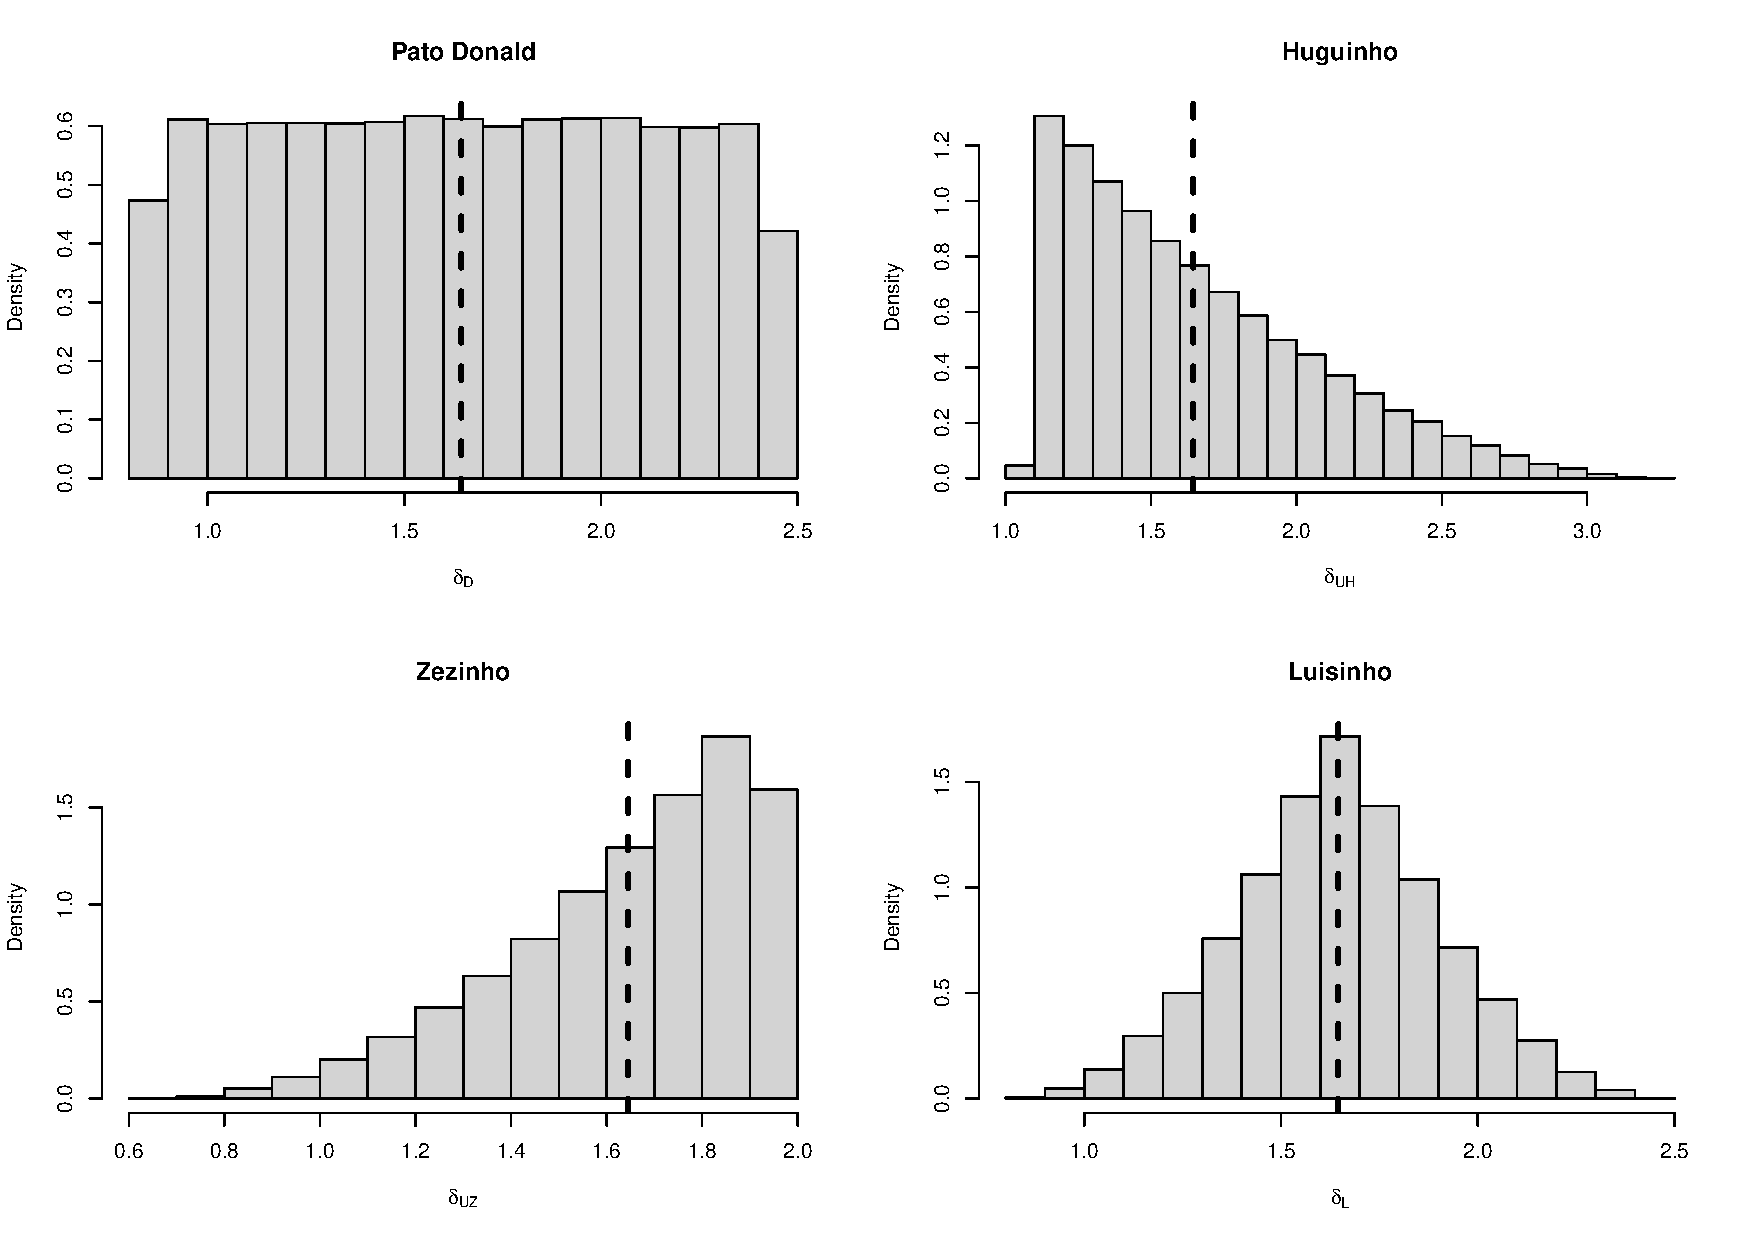
\includegraphics[scale=0.4]{ests_Q4.pdf}    
\end{center}
\caption{\textbf{Distribuição dos estimadores considerados pelos patos}.
Mostramos a distribuição de cada estimador com $\theta = \pi^2/6$, $n = 3$ e $M = 10^5$ realizações.
}
\label{fig:duck_ests}
\end{figure}
$\blacksquare$
}

\newpage
\section*{5.Questão bônus: Boss is boss, ain't it, dad?}

Considere mais uma vez o problema da questão 4.
Desta vez, Tio Patinhas resolveu propor o próprio estimador, e quer mostrar que esse estimador pode ser melhor que qualquer um dos propostos 
anteriormente.
Para isso, propõe utilizar um estimador da forma
$$
\delta_{\text{P}}(\bX) = (1-\alpha) \delta_{\text{UH}}(\bX) + \alpha \delta_{\text{UZ}}(\bX),
$$
com $\alpha \in (0, 1)$.
\begin{enumerate}[label=\alph*)]
 \item (10 pontos) Mostre que $\delta_{\text{P}}$ é não-viesado e compute seu erro quadrático médio;
 
 \textit{Dica}: Lembre-se de que para $a,b \in \mathbb{R}$,
 $$\vr\left(aX + bY\right) = a^2\vr(X) + b^2\vr(Y) + 2ab\operatorname{Cov}(X, Y).$$
 \item (10 pontos) Encontre $\alpha_{\text{op}}$ que faz com que $\delta_{\text{P}}$ tenha variância mínima.
 O estimador $\delta_{\text{P}}^{\text{op}}(\bX) = (1-\alpha_{\text{op}}) \delta_{\text{UH}}(\bX) + \alpha_{\text{op}} \delta_{\text{UZ}}(\bX)$ domina todos aqueles derivados na questão 4? Justifique.
\end{enumerate}
\textcolor{red}{\textbf{Conceitos trabalhados}: variância mínima, combinação convexa de estimadores não-viesados.}
\\
\textcolor{purple}{\textbf{Nível de dificuldade}: médio.}
\\
\textcolor{blue}{
\textbf{Resolução:}
Começamos mostrando que
\begin{align*}
 E[\delta_{\text{P}}(\bX)] &= E[(1-\alpha)\delta_{\text{UH}} + \alpha\delta_{\text{UZ}}],\\
 &= (1-\alpha)E[\delta_{\text{UH}}] + \alpha E[\delta_{\text{UZ}}],\\
 &= (1-\alpha)\theta + \alpha\theta = \theta.
\end{align*}
Portanto,
\begin{align*}
  R_{\alpha}(\theta, \delta_{\text{P}}(\bX)) &= \vr\left((1-\alpha)\delta_{\text{UH}} + \alpha\delta_{\text{UZ}}\right),\\
  &= \vr\left(\frac{(1-\alpha)}{k_{\text{H}}}\delta_{\text{H}} + \frac{\alpha}{k_{\text{Z}}}\delta_{\text{Z}}\right),\\
  &= \frac{(1-\alpha)^2}{k_{\text{H}}^2}\vr\left(m\right) + \frac{\alpha^2}{k_{\text{Z}}^2}\vr\left(M\right) + 2 \frac{\alpha(1-\alpha)}{k_{\text{H}}k_{\text{Z}}}\operatorname{Cov}(m, M),\\
  &= \gamma\left(\frac{(1-\alpha)^2n}{k_{\text{H}}^2}+ \frac{\alpha^2n}{k_{\text{Z}}^2}+ 2 \frac{\alpha(1-\alpha)}{k_{\text{H}}k_{\text{Z}}}\right),
\end{align*}
onde $\gamma = \operatorname{Cov}(m, M) = \frac{\theta^2}{(n+1)^2(n+2)}$.
\\
Para reponder b), vamos minimizar $ R_{\alpha}(\theta, \delta_{\text{P}}(\bX))$ com respeito a $\alpha$:
\begin{align}
\label{eq:Rd1}
 \frac{d}{d\alpha}  R_{\alpha}(\theta, \delta_{\text{P}}(\bX)) &= 2\gamma\left(\dfrac{\left(\left(k_{\text{Z}}^2+k_{\text{H}}^2\right)n-2k_{\text{H}}k_{\text{Z}}\right)\alpha-k_{\text{Z}}^2n+k_{\text{H}}k_{\text{Z}}}{k_{\text{H}}^2k_{\text{Z}}^2}\right),
\end{align}
Igualando (\ref{eq:Rd1}) a zero, obtemos
\begin{align*}
  \alpha_{\text{op}} &= \dfrac{k_{\text{Z}}^2n-k_{\text{H}}k_{\text{Z}}}{\left(k_{\text{Z}}^2+k_{\text{H}}^2\right)n-2k_{\text{H}}k_{\text{Z}}},\\
  &= \frac{9n+3}{10n+6}.
\end{align*}
Com isso, concluímos que o estimador do Tio Patinhas é melhor que os outros, finalizando a questão.
Como um extra, podemos calcular, depois de alguma álgebra,  
\begin{equation*}
 R_{\alpha}(\theta, \delta_{\text{P}}(\bX)) = \frac{2}{(5n+3)(n+2)}\theta^2.
\end{equation*}
É importante notar que a melhoria não é escandalosa. 
Por exemplo, para $\theta = \pi^2/6$, $n = 3$, $R_{\alpha}(\theta, \delta_{\text{UZ}}(\bX)) = 1.22 \times 10^{-3}$, enquanto $R_{\alpha}(\theta, \delta_{\text{P}}(\bX)) = 1.10 \times 10^{-3}$.
}
\bibliographystyle{apalike}
\bibliography{refs}

\end{document}
